\documentclass{article}
\usepackage{fancyhdr}
\usepackage{extramarks}
\usepackage{amsmath}
\usepackage{amsthm}
\usepackage{amsfonts}
\usepackage{tikz}
\usepackage[plain]{algorithm}
\usepackage{algpseudocode}
\usepackage{listings} 
\usepackage{neuralnetwork}
\usetikzlibrary{automata,positioning}

\usepackage{color}

\definecolor{dkgreen}{rgb}{0,0.6,0}
\definecolor{gray}{rgb}{0.5,0.5,0.5}
\definecolor{mauve}{rgb}{0.58,0,0.82}

\lstset{frame=tb,
  language=Python,
  aboveskip=3mm,
  belowskip=3mm,
  showstringspaces=false,
  columns=flexible,
  basicstyle={\small\ttfamily},
  numbers=none,
  numberstyle=\tiny\color{gray},
  keywordstyle=\color{blue},
  commentstyle=\color{dkgreen},
  stringstyle=\color{mauve},
  breaklines=true,
  breakatwhitespace=true,
  tabsize=3
}
%
% Basic Document Settings
%

\topmargin=-0.45in
\evensidemargin=0in
\oddsidemargin=0in
\textwidth=6.5in
\textheight=9.0in
\headsep=0.25in

\linespread{1.1}

\pagestyle{fancy}
\lhead{\hmwkAuthorName}
\chead{\hmwkClass\: \hmwkTitle}
\rhead{\firstxmark}
\lfoot{\lastxmark}
\cfoot{\thepage}

\renewcommand\headrulewidth{0.4pt}
\renewcommand\footrulewidth{0.4pt}

\setlength\parindent{0pt}

%
% Create Problem Sections
%

\newcommand{\enterProblemHeader}[1]{
    \nobreak\extramarks{}{Task \arabic{#1} continued on next page\ldots}\nobreak{}
    \nobreak\extramarks{Task \arabic{#1} (continued)}{Problem \arabic{#1} continued on next page\ldots}\nobreak{}
}

\newcommand{\exitProblemHeader}[1]{
    \nobreak\extramarks{Task \arabic{#1} (continued)}{Problem \arabic{#1} continued on next page\ldots}\nobreak{}
    \stepcounter{#1}
    \nobreak\extramarks{Task \arabic{#1}}{}\nobreak{}
}

\setcounter{secnumdepth}{0}
\newcounter{partCounter}
\newcounter{homeworkProblemCounter}
\setcounter{homeworkProblemCounter}{1}
\nobreak\extramarks{Task \arabic{homeworkProblemCounter}}{}\nobreak{}

%
% Homework Problem Environment
%
% This environment takes an optional argument. When given, it will adjust the
% problem counter. This is useful for when the problems given for your
% assignment aren't sequential. See the last 3 problems of this template for an
% example.
%
\newenvironment{homeworkProblem}[1][-1]{
    \ifnum#1>0
        \setcounter{homeworkProblemCounter}{#1}
    \fi
    \section{Task \arabic{homeworkProblemCounter}}
    \setcounter{partCounter}{1}
    \enterProblemHeader{homeworkProblemCounter}
}{
    \exitProblemHeader{homeworkProblemCounter}
}

%
% Homework Details
%   - Title
%   - Due date
%   - Class
%   - Section/Time
%   - Instructor
%   - Author
%

\newcommand{\hmwkTitle}{Lab\ \#3}
\newcommand{\hmwkDueDate}{September 25, 2019}
\newcommand{\hmwkClass}{CSCI964 Computational Intelligence}
\newcommand{\hmwkClassTime}{3.5}
\newcommand{\hmwkClassInstructor}{Zhifeng Wang}
\newcommand{\hmwkAuthorName}{\textbf{Mei Wangzhihui}}
\newcommand{\hmwkAuthorNum}{\textbf{2019124044}}
%
% Title Page
%

\title{
    \vspace{2in}
    \textmd{\textbf{\hmwkClass:\ \hmwkTitle}}\\
    % \normalsize\vspace{0.1in}\small{Due\ on\ \hmwkDueDate\ at 3:10pm}\\
    % \vspace{0.1in}\large{\textit{\hmwkClassInstructor\ \hmwkClassTime}}
    \vspace{3in}
}

\author{\hmwkAuthorName\ \hmwkAuthorNum}
\date{}

\renewcommand{\part}[1]{\textbf{\large Part \Alph{partCounter}}\stepcounter{partCounter}\\}

%
% Various Helper Commands
%

% Useful for algorithms
\newcommand{\alg}[1]{\textsc{\bfseries \footnotesize #1}}

% For derivatives
\newcommand{\deriv}[1]{\frac{\mathrm{d}}{\mathrm{d}x} (#1)}

% For partial derivatives
\newcommand{\pderiv}[2]{\frac{\partial}{\partial #1} (#2)}

% Integral dx
\newcommand{\dx}{\mathrm{d}x}

% Alias for the Solution section header
\newcommand{\solution}{\textbf{\large Solution}}

% Probability commands: Expectation, Variance, Covariance, Bias
\newcommand{\E}{\mathrm{E}}
\newcommand{\Var}{\mathrm{Var}}
\newcommand{\Cov}{\mathrm{Cov}}
\newcommand{\Bias}{\mathrm{Bias}}

\begin{document}

\maketitle

\pagebreak

\begin{homeworkProblem}
\lstset{language=C}
\begin{lstlisting}
    import numpy as np
    import random
    import matplotlib.pyplot as plt
    import matplotlib.animation as animation
    
    
    def sigmoid(x):
        return 1.0 / (1.0 + np.exp(-x))
    
    
    def numToVector(x, label_num):
        result = np.empty((1, label_num))
        result[x] = 1
        return result
    
    
    def readData(filepath, ifShuffle, feature_num=4):
        label_dict = {}
        xs = []
        ys = []
        ynums = []
        label_num = 0
        with open(filepath) as f:
            lines = f.readlines()
            if ifShuffle:
                random.shuffle(lines)
            for line in lines:
                x = list(map(float, line.split(',')[0:feature_num]))
                xs.append(np.array(x).reshape(feature_num, 1))
                label_str = line.strip('\n').split(',')[-1]
                if not label_str in list(label_dict.keys()):
                    label_num += 1
                    label_dict[label_str] = label_num
                ynums.append(label_dict[label_str])
            for ynum in ynums:
                y = np.zeros(label_num)
                y[ynum - 1] = 1.0
                ys.append(y.reshape(label_num, 1))
        return xs, ys
    
    
    class mlp(object):
        def __init__(self, lr=0.1, momentum=0.5, te=1e-5, epoch=100, size=None):
            self.learningRate = lr
            self.thresholdError = te
            self.maxEpoch = epoch
            self.size = size  # The number of neutron in every layer
            self.momentum = momentum
            self.W = []
            self.b = []
            self.last_dW = []
            self.last_db = []
            self.init()
    
        def init(self):
            #Initailize the Weight and Bias Matrix
            for i in range(len(self.size) - 1):
                self.W.append(np.mat(np.random.uniform(-0.5, 0.5, size=(self.size[i + 1], self.size[i]))))
                self.b.append(np.mat(np.random.uniform(-0.5, 0.5, size=(self.size[i + 1], 1))))
    
        # w: len(a[i+1]) x len (a[i]) a[i]: len(a[i]) x 1
        def forwardPropagation(self, item=None):
            a = [item]
            for i in range(len(self.W)):
                a.append(sigmoid(self.W[i] * a[-1] + self.b[i]))
            return a
    
        def backPropagation(self, label=None, a=None):
            # print("backPropagation--------------------begin")
            delta = []
            factor = 0.999999
            # Output layer gradient
            delta.append(np.multiply((a[-1] - label), np.multiply(a[-1], (1.0 - a[-1]))))
            for i in range(len(self.W) - 1):
                pd_ol = np.multiply(a[-2 - i], 1 - a[-2 - i])  # current layer gradient
                delta_hl = np.multiply(self.W[-1 - i].T * delta[-1], pd_ol)  # last gradient propagate to this layer * current layer gradient => error gradient to this layer
                delta.append(delta_hl)  # delta[0..len(selfW)-2] =>the last layer gradient to the 2nd layer gradient
            # if no W => the first bp, no last momentum.
            #self.learningRate = self.learningRate * factor
            if not len(self.last_dW):
                for i in range(len(self.size) - 1):
                    self.last_dW.append(np.mat(np.zeros_like(self.W[i])))
                    self.last_db.append(np.mat(np.zeros_like(self.b[i])))
                # Update the Weights
                for j in range(len(delta)):
                    # the gradient to the weights
                    ads = delta[j] * a[-2 - j].T
                    self.W[-1 - j] = self.W[-1 - j] - self.learningRate * ads  #W-lr*delta_W
                    self.b[-1 - j] = self.b[-1 - j] + self.learningRate * delta[j]  #b-lr*delta_b
                    self.last_dW[-1 - j] = self.learningRate * ads  # Record the direction of the update to add momentum
                    self.last_db[-1 - j] = self.learningRate * delta[j]
            else:
                for j in range(len(delta)):
                    ads = delta[j] * a[-2 - j].T
                    self.W[-1 - j] = self.W[-1 - j] - (self.learningRate * ads - self.momentum * self.last_dW[-1 - j])
                    self.b[-1 - j] = self.b[-1 - j] + (self.learningRate * delta[j] - self.momentum * self.last_db[-1 - j])
                    self.last_dW[-1 - j] = self.learningRate * ads - self.momentum * self.last_dW[-1 - j]
                    self.last_db[-1 - j] = self.learningRate * delta[j] - self.momentum * self.last_db[-1 - j]
    
            error = sum(0.5 * np.multiply(a[-1] - label, a[-1] - label))  #L2 loss
            return error
    
        def train(self, input_=None, target=None, show=10):
            epoch_errors = []
            cnt = 0
            for ep in range(self.maxEpoch):
                error = []
    
                for i in range(len(input_)):
                    a = self.forwardPropagation(input_[i])
                    e = self.backPropagation(target[i], a)
                    error.append(e[0, 0])
                epoch_error = sum(error) / len(error)
                epoch_errors.append(epoch_error)
                cnt = cnt + 1
                if len(epoch_errors) >= 2 and (abs(epoch_errors[-1] - epoch_errors[-2])) < self.thresholdError:
                    print("Finish {0}: {1}".format(ep, epoch_error))
                    break
                elif ep % show == 0:
                    print("epoch {0}: {1} ".format(ep, epoch_error, self.learningRate))
    
            plt.xlabel('epoch')
            plt.ylabel('loss')
            plt.title('epoch-loss \n learning rate={0} momentum={1} threshold error={2}'.format(self.learningRate, self.momentum, self.thresholdError))
            x = list(range(cnt))
            y = epoch_errors
            plt.plot(x, y)
            plt.show()
    
        def sim(self, inp=None):
            return self.forwardPropagation(item=inp)[-1]
    
    
    if __name__ == "__main__":
        x, y = readData('../iris.txt', False, 4)
        model = mlp(lr=0.1, momentum=0.3, te=1e-5, epoch=10000, size=[len(x[0]), 4, len(y[0])])
        model.train(x, y, 10)
    
\end{lstlisting}

Set initail $W = (0,0,0)$ initial $\theta = 0$ max $\delta_{error}=1E-9$ learning rate $LR=0.01$ 
\begin{figure}[]
	\centering
	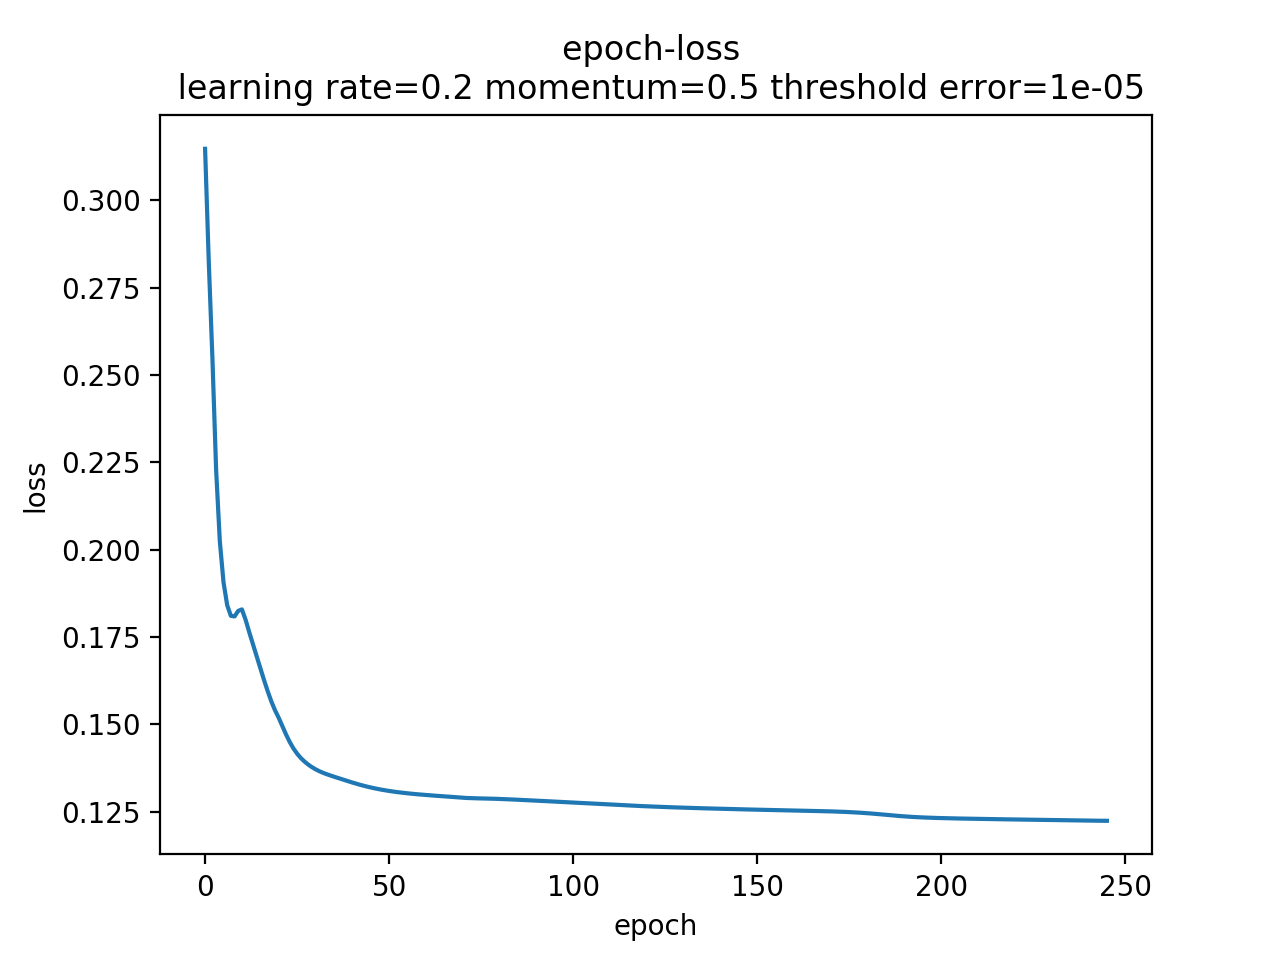
\includegraphics[width=1.0\textwidth]{image/Figure_1}
	\caption{Epoch-loss graph}
\end{figure}

% \begin{figure}[H]
% 	\centering
% 	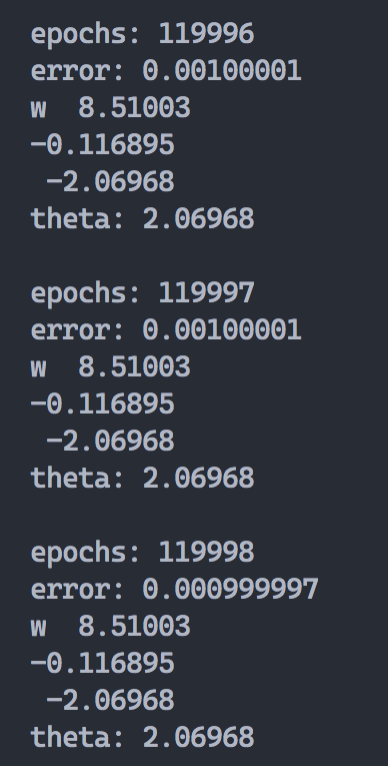
\includegraphics{image/100batch}
% 	\caption{Batch Method (batchsize = 100)}
% \end{figure}

\begin{figure}[]
	\centering
	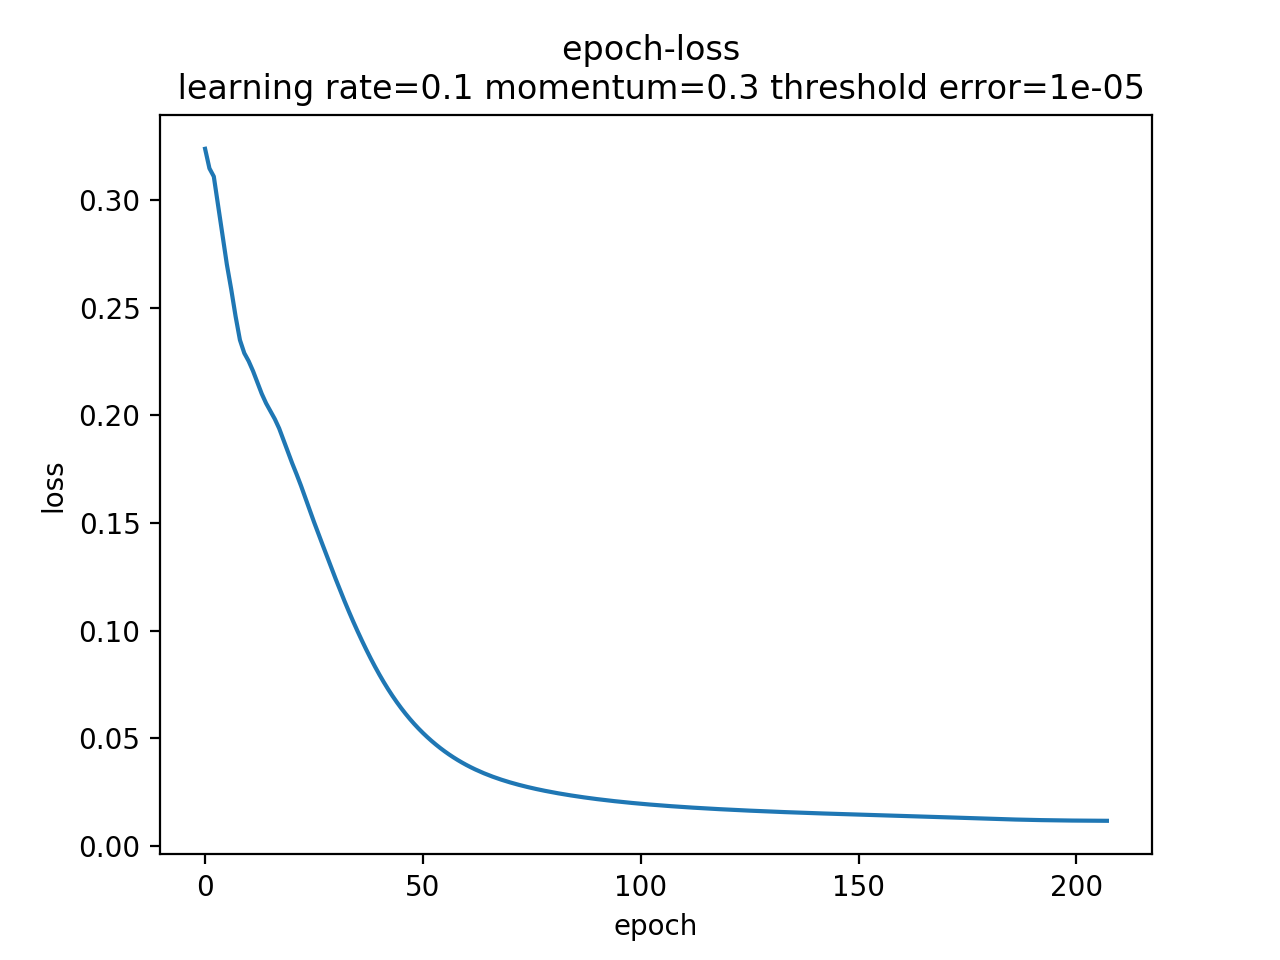
\includegraphics[width=1.0\textwidth]{image/Figure_2}
	\caption{Epoch-loss graph}
\end{figure}

\end{homeworkProblem}

\end{document}
